%%%%%%%%%%%%%%%%%%%%%%%%%%%%%%%%%%%%%%%%%%%%%%%%%%%
%% P3: Phenomenology of Particle Physics                         
%%
%% Author:  André Rubbia                   		 
%%
%% Figure 27.19 Precision measurements of the $Z^0$ asymmetry parameter ${\cal A}_e$.
%%
%% This work is licensed under the Creative Commons Attribution 4.0 International License. 
%% To view a copy of this license, visit http://creativecommons.org/licenses/by/4.0/ or 
%% send a letter to Creative Commons, PO Box 1866, Mountain View, CA 94042, USA.
%%
%%%%%%%%%%%%%%%%%%%%%%%%%%%%%%%%%%%%%%%%%%%%%%%%%%%

\documentclass[a4paper,10pt]{article}

\usepackage[T1]{fontenc}
\usepackage[utf8]{inputenc}
\usepackage{lmodern}
\usepackage[labelfont=bf]{caption}
\usepackage{upgreek}

\usepackage{tikz}
\usepackage{pgfplots}
\pgfplotsset{compat=1.17}
\usepgfplotslibrary{ternary}
\usepgfplotslibrary{fillbetween}
\usepgfplotslibrary{external}

\def\d{\mathrm{d}}
\setlength{\oddsidemargin}{-1.0cm}
\setlength{\evensidemargin}{-1.0cm}
\setlength{\textheight}{25cm}
\setlength{\textwidth}{18cm}

\pgfkeys{/pgf/number format/.cd,1000 sep={}}

\begin{document}

%%%%%%%%%%%%%%%%   FIGURE  %%%%%%%%%%%%%%%%%%%%%%%%%%%%%%
\begin{figure}[htb]
 	\centering
		\begin{tikzpicture}[scale=1]
%
% Ae
%
\begin{axis}[
    xbar,
    width=10cm,
    height=4cm,
    title={Asymmetry parameter ${\cal A}_e$},
    xlabel={${\cal A}_e$},
    symbolic y coords={ybot,average,SLD,OPAL,L3,DELPHI,ALEPH,ytop},
    ytick=data,
    ymin=ybot,ymax=ytop,
    xmin=0.1, xmax=0.2,
    legend pos=north east,
]
\addplot[
    color=blue,only marks,
    mark=*,
        error bars/.cd,
    x dir=both, x explicit
    ]
    coordinates {
    (0.1504,ALEPH)+-(0.0068469,0)
    (0.1382,DELPHI)+-(0.0116108,0)
    (0.1678,L3)+-(0.0130495,0)
    (0.1454,OPAL)+-(0.0113842,0)
    (0.1516,SLD)+-(0.0021,0)
    (0.1515,average)+-(0.0019,0)
};
    \draw[gray,fill,fill opacity=0.2] (axis cs:0.1496,ybot) rectangle (axis cs:0.1534,ytop);
\end{axis}
\end{tikzpicture}
	\caption{Precision measurements of the $Z^0$ asymmetry parameter ${\cal A}_e$.
		The average value is from the PDG.}
\end{figure}
%
%%%%%%%%%%%%%%%%   END FIGURE  %%%%%%%%%%%%%%%%%%%%%%%%%%%%%%
%


\end{document}
